\subsection{Rigid bodies}
	\cite{lecRigidBodies} To simulate the translational motion of a rigid body it is sufficient to simulate the motion of the center of mass. As the vertices stay motionless relative to the center the position of every vertex can be calculated easily from the position of the center. 
	If the motion is arbitrary it can still be represented by just a translational and a rotational movement. 
	The simulation is done by a rigid body simulator, which needs the following parameters:
	\begin{itemize}
		\item densitiy $\rho$ and mass $m$
		\item the moment of inertia, which is (in the bodie's frame of reference) constant to each body and behaves to rotational movement, as mass behaves to translational movement.
		\item linear position $\bm{x}\in\mathbb{R}^{3}$ and momentum $\bm{p}\in\mathbb{R}^{3}$
		\item orientation $\bm \Omega\in\mathbb{R}^{3}$ and angular momentum $\bm L\in\mathbb{R}^{3}$
		\item coefficient of restitution $C_r$, which stores the ratio between elastic and non elastic collision
	\end{itemize}
	
\subsection{Skinning}
	It is very costy to provide physically correct positions for every single vertex. So a method named skinning is used. So called bones are added to the mesh (rigging) and every vertex is assigned to one or more bones. And similarly to real bones the vertices follow the movement of the bone they are attached to. To prevent artifacts a vertex can not only be assigned to one bone, but to multiple bones with weighting. \\
	The bones behave like rigid bodies they can be moved and rotated, but they do not change their form. For example: In a model of an arm, the bones would be placed like to the bones in a real arm and if the bones move, the vertices follow. A vertex at the elbow would be associated with the bone of the upper and of the lower arm, and it's movement is a linear combination of the movement of the bones. So the vertex follows the movement of both bones. This gives an artist the opportunity to modify a mesh very easily. \\
	For a mesh with $N$ vertices and $B$ bones some more values have to be stored.
\begin{itemize}
	\item undeformed mesh vertex positions: $\bm{u} \in \mathbb{R}^{N \times 3}$	
	\item skinning weights: $\bm{W} \in \mathbb{R} ^{N \times B}$
	\item the desired transformation, which consist of:
		\subitem rotation: $\bm{R} \in \mathbb{R}^{B\times 3\times 3}$
		\subitem translation: $\bm{T}\in \mathbb{R}^{B\times 3}$
\end{itemize}
	The skinning weight matrix $\bm{W}$ contains a row for each vertex and a column for each bone. The value $W_{ib}$ represents how much percent of the movement of bone $b$ affects vertex $\bm x$.\\
	So to get the transformed position of a single vertex we apply the weighted transformation of each bone on the vertex.
\begin{align}
\bm{x}_i =\sum_{b\in B} \bm{W}_{ib}\left(\bm{T}_b +\bm{R}_b \bm{u}_i\right)
\end{align}
As we want to use $E$ example poses on every vertex we don't have one desired Transformation, but one for every pose, generated by the artist. So we extend $\bm{R}$ and $\bm{T}$ by one dimension for the examples and add a matrix that contains, how much every example pose acts on every vertex:
\begin{itemize}
	\item $\bm {R}\in\mathbb{R}^{B\times E\times 3\times 3}$
	\item $\bm {T}\in \mathbb{R}^{B\times E\times 3}$
	\item $\bm{E}\in \mathbb{R}^{N \times E}$
\end{itemize}

We have to somehow consider mutliple example poses. The intuuitive approach is to use linear interpolation and weight the individual transformations with the weighting matrix $\bm{E}$. We now can determine the new position of each vertex by:
\begin{align}
\bm{x}_i = \sum_{b\in B}\bm{W}_{ib}\left( \sum_{e=1}^{E} \bm{E}_{ie} \left( \bm{T}_b + \bm{R}_{be} \bm{u}_i \right) \right) 
\end{align}
With the translational part this works fairly well, however linear interpolation does not work well on rotation matrices. This is due to the fact, that a 3 dimensional rotation has 3 degrees of freedom, while a rotation matrix has 9 entries. So 6 Entries are somehow redundant and have to be bound via constraints (orhogonality and determinant is 1). So if we linearly interpolate each single entry of a roation matrix it is not guaranteed, that the resulting matrix is itself a rotation matrix. Quaternion rotation provides a solution to this.
\subsubsection{Quaternion rotation and QLERP}
Ken Shoemake presented a method to use quarternions for a 3 dimensional rotation instead of a matrix \cite{Quat}.
Quaternions are an extension of the complex numbers. They have 3 imaginary units and are based on the identity
\begin{align}
i^2=j^2=k^2=ijk=-1
\end{align}
Each quaternion has the form: $a+ bi+cj+dk$.
Standard algebraic operations on quaternions can be determined by using the standard form. For example addition:
\begin{align}
\bm p &= a+ bi+cj+dk\\
\bm q &= x+ yi + zj+wk\\
\bm p+ \bm q &= (a+ x) + (b+y)i + (c+z)j + (d+w)k
\end{align}
The length is:
\begin{align}
||\bm p|| = \sqrt{a^2+b^2+c^2+d^2}
\end{align}
How exactly a quaternion can be used to rotate a vector can be read in \cite{Quat}.\\
Quaternion rotation has a main advantage over matrix rotation. Having 3 degrees of freedom in a 3D rotation and 4 entries in a quaternion there is only one additional entry, instead of 6. So only one constraint is needed to provide a valid rotation. It turns out that a rotation quaternion has to be of length one, a constraint that is easy to fulfill.\\
So to interpolate between two rotations it is sufficient to linearly interpolate between the two rotation quaternions and normalize them afterwards. \cite{QLERP}
The formula for interpolation of the rotation quaternions $\bm q$ and $\bm p$ with the parameter $t \in[0,1]$ the following formula is used:
\begin{align}
l(t;\bm{p},\bm{q}) = \frac{(1-t)\bm{p} + t\bm{q}}{||(1-t)\bm{p} + t\bm{q}||}
\end{align}
However it should be noted that the interpolation provides no constant speed, considering the distance on the rotation circle. As seen in Figure \ref{fig:image} a change at the beginning or end moves the point E on the circle further than at the middle. This effect however is small and therefore disregarded, as the exact solution, provided in \cite{Quat} would be far more computational complex \cite{QLERP}.
To blend multiple rotations we now use a matrix, containing the quaternion values for each example pose $\bm{R}^{4\times E}$ and the weightings $\bm{E}^{N\times E}$. This works, because the columns of $\bm{E}$ sum up to 1.
\begin{align}
\bm{R}_i' =\text{QLERP} (\bm{E}_i,\bm{R}) = \text{normalize} \left( \sum_{e\in E} \bm{E}_{ie} \bm{R}_{e}\right)
\end{align}


\begin{figure}[tb]
	\centering
	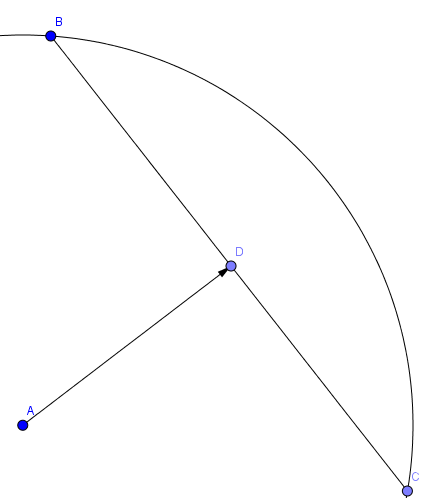
\includegraphics[width=0.3\linewidth]{images/quatrot1} 
	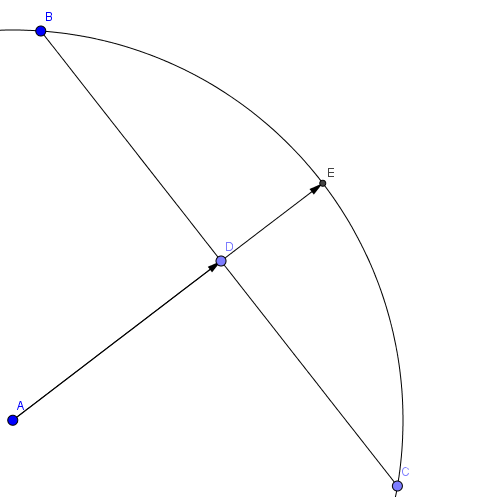
\includegraphics[width=0.33\linewidth]{images/quatrot2} 
	\caption{\label{fig:image} On the left: Idea, how linear interpolation between rotation matrices looks. If linear interpolation between the two points $B$ and $C$ on a circle is used, the resulting point does not lie on the circle. On the right: Interpolating with quaternions. The result can be easily mapped onto the sphere by normalizing the quaternion.
	}
\end{figure}


\subsection{Recap Skinning}
Now we have a method to deform meshes with the help of bones and to blend in given example poses.
The input consists of the constant data:
\begin{itemize}
\item The Vertex positions in undeformed state: $\bm u\in\mathbb{R}^{N\times 3}$
\item The weighting of each bone for the vertcies: $\bm W\in\mathbb{R} ^{N \times B}$
\item The transformation for each example pose and bone, consisting of
	\subitem The rotational part $\bm R\in\mathbb{R}^{B\times 4\times  E}$
	\subitem The translational part $\bm T\in\mathbb{R}^{B \times 3\times E}$
\end{itemize}
and the changing data:
\begin{itemize}
	\item example Weights $\bm{E}\in\mathbb{R}^{N\times E}$
\end{itemize}
Let $\text{rotate} (\bm{q},\bm{x})$ be the function that rotates the position $\bm{x}$ by the quaternion $\bm{q}$.
The translational part is interpolated linearly, the rotational by the $QLERP$-algorithm.
The skinned mesh vertex positions $\bm{x} \in \mathbb{R}^{N\times 3}$ can now be calculated by:
\begin{align}
\bm{x}_i = \sum_{b\in B} \bm{W}_{ib}\left(\sum_{e=1}^{E}\bm{E}_{ie}\bm{T}_{be} + \text{rotate}(\text{QLERP}(\bm{E}_i,\bm{R}_b),\bm{u}_i)\right)
\end{align}
